\documentclass[journal]{IEEEtran}

\usepackage[T1]{fontenc}
\usepackage[utf8]{inputenc}
\usepackage{amsmath,amssymb,amsfonts}
\usepackage{graphicx}
\usepackage{booktabs}
\usepackage{array}
\usepackage{url}
\usepackage{xcolor}
\usepackage[hidelinks]{hyperref}
\usepackage{orcidlink}
\usepackage{balance}

\graphicspath{{../figures/}}

\renewcommand{\topfraction}{0.92}
\renewcommand{\bottomfraction}{0.75}
\renewcommand{\textfraction}{0.08}
\renewcommand{\floatpagefraction}{0.80}

% IEEEtran hard-codes an em-dash after the abstract and index-terms names; the CAOS
% content standard (ADR-0067) excludes em-dashes, so the separator is a full stop.
\makeatletter
\def\abstract{\normalfont
    \if@twocolumn
      \@IEEEabskeysecsize\bfseries\textit{\abstractname}.\ \relax
    \else
      \bgroup\par\addvspace{0.5\baselineskip}\centering\vspace{-1.78ex}\@IEEEabskeysecsize\textbf{\abstractname}\par\addvspace{0.5\baselineskip}\egroup\quotation\@IEEEabskeysecsize
    \fi\@IEEEgobbleleadPARNLSP}
\def\IEEEkeywords{\normalfont
    \if@twocolumn
      \@IEEEabskeysecsize\bfseries\textit{\IEEEkeywordsname}.\ \relax
    \else
      \bgroup\par\addvspace{0.5\baselineskip}\centering\@IEEEabskeysecsize\textbf{\IEEEkeywordsname}\par\addvspace{0.5\baselineskip}\egroup\quotation\@IEEEabskeysecsize
    \fi\@IEEEgobbleleadPARNLSP}
\makeatother

% Page-1 header block (conventions/manuscript-header-standard.md). The four document
% macros are set by the publishing tool when the version DOI is reserved.
\newcommand{\doctype}{Technical report}
\newcommand{\docversion}{v1.1}
\newcommand{\docdate}{18 September 2026}
\newcommand{\versiondoi}{10.5281/zenodo.22824355}
\newcommand{\conceptdoi}{10.5281/zenodo.21519481}
\newcommand{\docrepo}{github.com/fsantibanezleal/CAOS\_FragmentIQ}
\newcommand{\headerblock}{%
\begin{center}
\fbox{\parbox{0.94\textwidth}{\small\raggedright
\textbf{\doctype} \quad$\cdot$\quad \docversion, \docdate \quad$\cdot$\quad Licence CC BY 4.0\\[2pt]
CAOS open-research programme \quad$\cdot$\quad CAOS\_FragmentIQ, image-based muckpile fragmentation analysis\\[2pt]
Version DOI \href{https://doi.org/\versiondoi}{\texttt{\versiondoi}} \quad$\cdot$\quad
concept DOI (always latest) \href{https://doi.org/\conceptdoi}{\texttt{\conceptdoi}}\\[2pt]
Not peer reviewed. Source code, data and computational records: \href{https://\docrepo}{\texttt{\docrepo}}
}}
\end{center}}

\begin{document}

\title{FragmentIQ: The Systematic Bias of Image-Based\\ Muckpile Fragmentation Analysis,\\ and Its Correction}

\author{Felipe~Santiba\~nez-Leal~\orcidlink{0000-0002-0150-3246}%
\thanks{F. Santiba\~nez-Leal is with the CAOS open-research programme, Santiago, Chile
(e-mail: fsantibanez@gmail.com; ORCID 0000-0002-0150-3246).}%
\thanks{Interactive tool and reproducible pipeline (MIT) at
\url{https://github.com/fsantibanezleal/CAOS_FragmentIQ}; the tool is available at
\url{https://fragmentiq.fasl-work.com}.}}

% The leading {} lets IEEEtran's \MakeUppercase reach \doctype, so the whole head is set in capitals.
\markboth{{}\doctype\ \docversion, 2026}%
{Santiba\~nez-Leal: The systematic bias of image-based muckpile fragmentation analysis}

\IEEEaftertitletext{\vspace{-0.6\baselineskip}\headerblock\vspace{0.2\baselineskip}}

\maketitle

\begin{abstract}
The size distribution of a blasted muckpile sets the energy cost of every downstream crushing and grinding stage,
and it is routinely estimated by photographing the muckpile and analysing the image. The biases of this image-based
granulometry are known qualitatively but rarely measured, because the true size distribution of a real muckpile is
unknown. FragmentIQ measures them on synthetic muckpiles whose true fragmentation is known by construction, using
the threshold and marker-controlled watershed delineation of the standard tools. Over seven cases the watershed finds
$1.5$ to $2.5$ times as many fragments as exist, and the recovered $P_{50}$ and $P_{80}$ fall below the truth in
every case, by $16.5$--$31.5\%$ and $13.5$--$27.6\%$. About half of the shortfall is present before delineation: a
perfect delineation of the ground-truth label map already recovers $P_{50}$ $7.9$--$15.8\%$ below the nominal size,
because the visible area of each fragment is smaller than its nominal diameter implies. The shortfall is
systematic. A learned multiplicative correction, predicted from four shape features of the recovered distribution,
reduces the mean $P_{50}$ error on 17 held-out muckpiles from $28.4\%$ to $3.98\%$. Refining the foreground with a
convolutional boundary classifier before the same watershed lowers the mean $P_{50}$ error on eight held-out
muckpiles only from $27.2\%$ to $23.8\%$, against $13.3\%$ for a perfect delineation. A raw image-based
fragmentation estimate is therefore biased fine by tens of percent; a size calibration against a known reference
removes most of that bias, and a better delineation cannot remove the part present before delineation.
\end{abstract}

\begin{IEEEkeywords}
Rock fragmentation, muckpile, particle size distribution, image analysis, watershed segmentation, Rosin-Rammler,
Kuz-Ram, blasting, calibration, synthetic ground truth.
\end{IEEEkeywords}

\section{Introduction}

\IEEEPARstart{T}{he} degree to which a drill-and-blast round fragments the rock, quantified as the particle-size
distribution of the resulting muckpile, is one of the most consequential numbers in a mine: a finer muckpile is
cheaper to dig, haul and, above all, crush and grind, so blast design is tuned to it, and predicting it from blast
parameters is the classic Kuz-Ram problem~\cite{kuznetsov,cunningham}. Measuring it after the fact, by sieving, is
impractical at production scale, so the standard practice is image-based granulometry: photograph the muckpile,
delineate the visible fragments, convert their areas to sizes, and fit a Rosin-Rammler distribution~\cite{rosin}.
Commercial systems such as WipFrag~\cite{maerz} and Split delineate the fragments by edge detection and watershed
segmentation~\cite{vincent}. Their error modes, the splitting of large blocks into several apparent fragments and the
loss of fines below the image resolution, are usually stated as caveats rather than measured, because the true
distribution of a real muckpile, against which the error would be measured, is not known.

FragmentIQ measures the error on synthetic muckpiles whose true fragmentation is known by construction. It runs the
threshold and watershed delineation of the classical tools, reads $P_{50}$ and $P_{80}$ off the recovered size
distribution, and compares them with the truth over seven cases that span coarse to fine and monosized to broad
distributions. It then separates the part of the shortfall that is present before delineation from the part the
delineation adds, measures how much of the shortfall a learned size correction removes, and tests whether refining
the foreground with a learned boundary classifier closes the gap. The contribution is a ground-truthed measurement of
the bias of the standard method, not a new fragmentation algorithm.

\section{Synthetic Muckpiles and the Measurement}\label{sec:method}

\emph{Scenes.} Each synthetic muckpile is a $560\times420$-pixel image of irregular polygonal fragments on a dark
background. Fragment diameters are drawn from a Rosin-Rammler distribution $P(x)=1-\exp[-(x/x_c)^n]$ with
characteristic size $x_c$ and uniformity index $n$. Each fragment is drawn as a polygon of $8$ to $11$ vertices at
$0.78$ to $1.12$ times its nominal radius, with its own grey level, radial shading and grain, and the fragments are
placed largest first so that they touch with little overlap, until the surface is full. The ground truth is the
generator's own record: the nominal diameter of every placed fragment and a per-pixel map of the fragment each pixel
belongs to. The seven cases (Table~\ref{tab:cases}) span three size regimes, the same medium muckpile under even and
under raking light (I-EVEN, I-SHADOW), a monosized control whose fragments all have a nominal diameter of
$120$~mm (C-MONO), and a known Rosin-Rammler target with $x_c=160$~mm and $n=1.7$ (C-KNOWN).

\emph{Classical pipeline.} The foreground is the set of pixels brighter than a fixed grey threshold ($58$ of $255$).
A chamfer distance transform of the foreground gives one marker per local maximum after non-maximum suppression, and
a marker-controlled flood in descending distance order labels the fragments and leaves ridges at their boundaries,
the watershed of~\cite{vincent} as the classical tools apply it. Each labelled region gives an equivalent-circle
diameter; the sizes form a mass-weighted cumulative passing curve, with mass proportional to the cube of the
diameter, and $P_{50}$ and $P_{80}$ are read off that curve by linear interpolation. A Rosin-Rammler fit is made to
the same curve. The true distribution is reduced in the same way from the nominal diameters.

\emph{Perfect delineation.} To separate the error of the delineation from what the image can show at all, the same
reduction is applied to the ground-truth label map: the equivalent-circle diameter of the pixels each fragment
occupies in the image. This is the distribution a delineation would recover if it found every visible fragment
exactly.

\emph{Learned size correction.} A small regression network, with one hidden layer of $16$ units, predicts a
multiplicative correction $k=P_{50}^{\mathrm{true}}/P_{50}^{\mathrm{rec}}$ from four features of the classical
recovery: the recovered $P_{50}$, the ratio $P_{80}/P_{50}$, the logarithm of the fragment count, and the passing
fraction at half the recovered $P_{50}$. It is trained on $39$ of $56$ synthetic muckpiles (four size regimes, two
lighting conditions and seven seeds, all disjoint from the seven cases) and evaluated on the remaining $17$.

\emph{CNN-refined foreground.} Learned delineation of rock fragments has been demonstrated with deep instance
segmentation~\cite{qiao}. Here a two-layer convolutional network classifies $16\times16$-pixel patches as
inter-fragment seam or fragment interior, and it is used only to refine the foreground that the same watershed
floods. It is trained on patches from the same $56$ muckpiles, seam-centred patches against deep-interior patches
with the ambiguous band between them excluded, and reaches a patch-level boundary F1 of $0.997$ on a held-out fifth
of the patches. The refined foreground is the thresholded foreground after a morphological closing, cut wherever the
network's seam probability reaches a threshold. The grey threshold and the seam threshold ($61$ and $0.7$) are
selected on eight tuning muckpiles, and the result is measured on eight test muckpiles with disjoint seeds (four size
regimes, two seeds each, even lighting).

\section{The Systematic Bias}\label{sec:bias}

\begin{figure*}[!t]
\centering
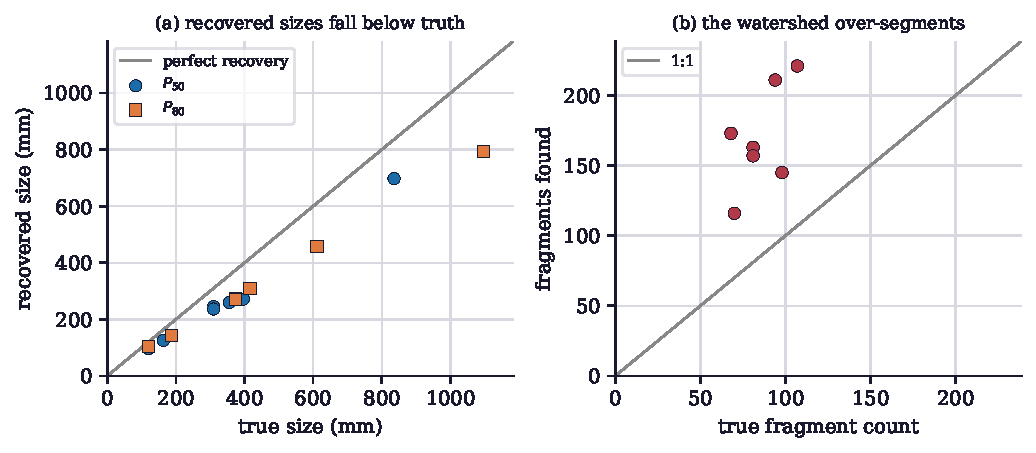
\includegraphics[width=0.86\textwidth]{fig-bias.pdf}
\caption{The bias of image-based fragmentation analysis, measured against known ground truth over seven synthetic
muckpiles. \textbf{(a)} Recovered versus true $P_{50}$ and $P_{80}$: every point falls below the line of perfect
recovery, so the pipeline reports sizes finer than the truth, by $16.5$--$31.5\%$ at $P_{50}$ and $13.5$--$27.6\%$ at
$P_{80}$. \textbf{(b)} Fragments found versus true fragment count: every point lies above the one-to-one line. The
watershed \emph{over-segments}, finding $1.5$ to $2.5$ times as many fragments as exist, which shifts the size
distribution fine.}
\label{fig:bias}
\end{figure*}

On every one of the seven synthetic muckpiles the recovered $P_{50}$ and $P_{80}$ fall below the true values
(Fig.~\ref{fig:bias}a, Table~\ref{tab:cases}): by $16.5$ to $31.5\%$ at $P_{50}$ (median $23.3\%$) and by $13.5$ to
$27.6\%$ at $P_{80}$ (median $25.5\%$). The largest absolute shortfall is at the coarse end, where the true $P_{80}$
of $1096$~mm in R-COARSE is recovered as $794$~mm. Raking light increases the $P_{50}$ shortfall of the same muckpile
from $20.9\%$ (I-EVEN) to $23.6\%$ (I-SHADOW), and even the monosized control C-MONO, whose true $P_{50}$ and $P_{80}$
are both $120$~mm, is recovered at $97$ and $104$~mm. The watershed \emph{over-segments} (Fig.~\ref{fig:bias}b): it
finds $1.5$ to $2.5$ times as many fragments as exist (median $2.0$), because the grain and shading inside a fragment
leave dark holes in the thresholded foreground, and each hole adds distance-transform maxima that seed extra regions.
More, smaller apparent fragments shift the size distribution fine.

\begin{table}[!t]
\centering
\caption{Recovered versus true fragmentation over the seven synthetic muckpiles ($x_c$, $n$: the Rosin-Rammler
parameters of the generator; t/r: true/recovered). The watershed finds more fragments than exist and recovers
$P_{50}$ and $P_{80}$ below truth in every case. I-SHADOW is the I-EVEN muckpile under raking light.}
\label{tab:cases}
\footnotesize
\begin{tabular}{@{}l c c c c@{}}
\toprule
Case & $x_c$ (mm), $n$ & found/true & $P_{50}$ t/r (mm) & $P_{80}$ t/r (mm) \\
\midrule
R-COARSE & $320$, $1.4$ & $116/70$  & $836/698$ & $1096/794$ \\
R-MEDIUM & $180$, $1.6$ & $145/98$  & $356/260$ & $416/310$ \\
R-FINE   & $90$, $1.9$  & $211/94$  & $164/126$ & $188/144$ \\
I-EVEN   & $180$, $1.6$ & $163/81$  & $310/245$ & $374/274$ \\
I-SHADOW & $180$, $1.6$ & $157/81$  & $310/237$ & $374/271$ \\
C-MONO   & $120$, mono  & $221/107$ & $120/97$  & $120/104$ \\
C-KNOWN  & $160$, $1.7$ & $173/68$  & $397/272$ & $611/458$ \\
\bottomrule
\end{tabular}
\end{table}

Over-segmentation is not the whole shortfall (Table~\ref{tab:decomp}). A perfect delineation of the ground-truth
label map already recovers $P_{50}$ $7.9$ to $15.8\%$ below the nominal truth (median $13.1\%$) and $P_{80}$ $7.7$
to $14.2\%$ below it (median $12.0\%$). Two properties of the scenes produce this part. Each fragment is drawn as a
polygon within $0.78$ to $1.12$ times its nominal radius, so its area is on average smaller than that of the nominal
circle, and fragments placed later overlap the edges of the earlier, larger ones, whose visible area shrinks
further. The delineation then adds $8.9$ to $18.6\%$ at $P_{50}$ (median $10.2\%$) and $6.3$ to $19.0\%$ at $P_{80}$
(median $14.7\%$) relative to the perfect delineation. A raw image-based $P_{50}$ is therefore an underestimate of
tens of percent, with one part that a better delineation can remove and one part that it cannot.

\begin{table}[!t]
\centering
\caption{Where the shortfall arises, in percent: the shortfall of a perfect delineation of the ground-truth label
map against the nominal truth (before delineation), and the further shortfall of the watershed against that perfect
delineation (added by delineation). The two compose multiplicatively into the shortfalls of
Table~\ref{tab:cases}.}
\label{tab:decomp}
\footnotesize
\begin{tabular}{@{}l c c c c@{}}
\toprule
 & \multicolumn{2}{c}{$P_{50}$ shortfall (\%)} & \multicolumn{2}{c}{$P_{80}$ shortfall (\%)} \\
\cmidrule(lr){2-3}\cmidrule(l){4-5}
Case & before & added & before & added \\
\midrule
R-COARSE & $7.9$  & $9.3$  & $10.5$ & $19.0$ \\
R-MEDIUM & $12.0$ & $17.1$ & $12.0$ & $15.3$ \\
R-FINE   & $14.6$ & $10.2$ & $11.2$ & $13.9$ \\
I-EVEN   & $13.1$ & $8.9$  & $14.2$ & $14.7$ \\
I-SHADOW & $13.1$ & $12.1$ & $14.2$ & $15.6$ \\
C-MONO   & $10.9$ & $9.5$  & $7.7$  & $6.3$  \\
C-KNOWN  & $15.8$ & $18.6$ & $14.0$ & $12.8$ \\
\bottomrule
\end{tabular}
\end{table}

\section{Correcting the Bias}\label{sec:correction}

\begin{figure*}[!t]
\centering
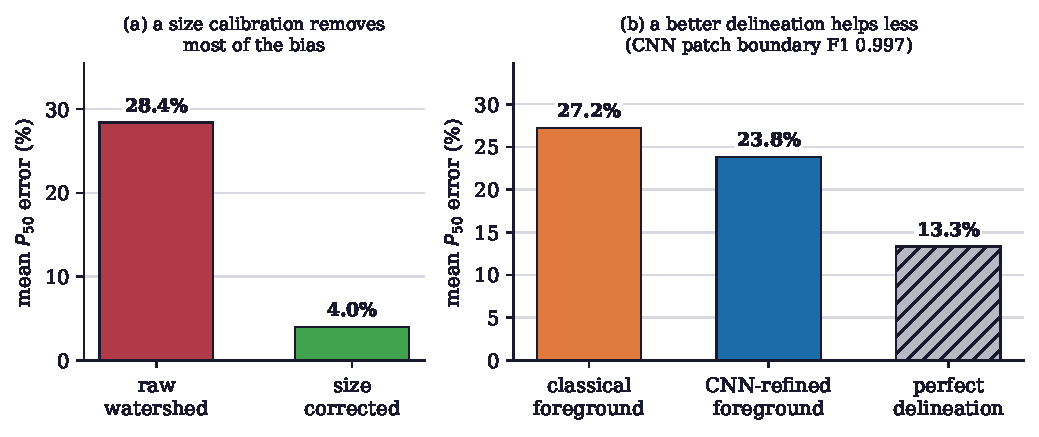
\includegraphics[width=0.86\textwidth]{fig-correction.pdf}
\caption{Correcting the bias. \textbf{(a)} Mean absolute $P_{50}$ error on 17 held-out muckpiles, for the classical
pipeline and after the learned size correction: from $28.4\%$ to $3.98\%$. \textbf{(b)} Mean absolute $P_{50}$ error
on eight held-out test muckpiles when the same watershed floods the classical foreground ($27.2\%$), the CNN-refined
foreground ($23.8\%$), or a perfect delineation of the ground-truth label map ($13.3\%$). The shortfall that a perfect
delineation leaves is present before delineation, so only the size correction removes it.}
\label{fig:correction}
\end{figure*}

Because the shortfall is systematic, it is largely correctable (Fig.~\ref{fig:correction}a). On the 17 held-out
muckpiles the learned size correction reduces the mean absolute $P_{50}$ error from $28.4\%$ for the classical
pipeline to $3.98\%$, a sevenfold reduction: the fine shift is consistent enough that one multiplicative factor,
adapted to the shape of the recovered distribution, largely undoes it. A better delineation helps less
(Fig.~\ref{fig:correction}b). On the eight test muckpiles the CNN-refined foreground lowers the mean $P_{50}$ error of
the same watershed from $27.2\%$ to $23.8\%$. A perfect delineation of the label map would still leave $13.3\%$ on
these muckpiles, because a correct segmentation cannot restore fragment area that the image does not show; the
refined foreground closes $3.4$ of the $13.9$ percentage points between the classical pipeline and that limit. The
size correction removes both parts at once, because it is fitted against the true size directly. In practice, the
size estimate should first be calibrated against a known reference, and a better segmentation is a secondary
improvement.

\section{Discussion and Scope}\label{sec:discuss}

Image-based fragmentation analysis by threshold and watershed delineation is biased fine, here by $16.5$ to $31.5\%$
at $P_{50}$ and $13.5$ to $27.6\%$ at $P_{80}$. Roughly half of the $P_{50}$ shortfall is present in the image before
any delineation, and over-segmentation adds the rest. A learned size correction removes most of it, taking the mean
$P_{50}$ error to about four percent, while a learned refinement of the foreground helps only modestly, and even a
perfect delineation leaves the first part. A raw muckpile image number is therefore an underestimate to
be calibrated, and the calibration, not the segmentation method, is where most of the accuracy is won.

The measurements have limits. All scenes are synthetic, used because their true size distribution is known and the
bias can therefore be measured, which is not possible on a real muckpile without independent sieving. The split of
the shortfall between the image and the delineation depends on how the generator draws fragments and on taking the
nominal diameter as the true size; on a photograph the reference is a sieve size, whose relation to the visible
outline differs. The held-out muckpiles of the size correction share the generator, size regimes and lighting of its
training muckpiles and differ only in seed, so $3.98\%$ is an in-distribution figure, and the patch F1 of the
boundary classifier is measured on patches drawn from its training scenes. The magnitudes are representative of the
mechanism, not a calibration transferable to a specific site, which would need its own ground-truthed reference.

\section{Conclusion}

Measured against ground truth on synthetic muckpiles, image-based fragmentation analysis by threshold and watershed
delineation is biased fine: it finds $1.5$ to $2.5$ times the true fragment count and recovers $P_{50}$ and $P_{80}$
$13.5$ to $31.5\%$ below truth. About half of the $P_{50}$ shortfall is present before delineation, in the visible
area of the fragments, and over-segmentation adds the rest. The bias is systematic, so a learned size correction
reduces the mean $P_{50}$ error from $28.4\%$ to $3.98\%$ on held-out muckpiles, while a learned refinement of the
foreground reduces it only from $27.2\%$ to $23.8\%$, against $13.3\%$ for a perfect delineation. Calibrating the
size estimate against a known reference, not improving the segmentation, is the dominant correction.

\appendices
\section{Reproduction}\label{app:repro}

The repository artifacts under \path{data/derived/} carry the seven cases' true and recovered size distributions
and fragment counts (\path{case-results.json}) and the learned-model metrics (\path{fq-learned.json}: the raw and
size-corrected $P_{50}$ errors, the classical and CNN-refined errors, and the boundary F1). The training, tuning and
test muckpiles are generated by \path{data-pipeline/pipeline/science/gen_train.mjs}; the two networks are trained by
\path{train_frag.py}, and the refined foreground is scored by \path{eval_frag.mjs}, both in the same folder. The
script \path{manuscripts/fragmentation/data/decompose.mjs} runs the same engine on the seven cases and the eight test
muckpiles and writes the shortfall decomposition (\path{decomposition.json}). The figure script under
\path{manuscripts/fragmentation/figures/} reads \path{fq.json} and \path{decomposition.json} from that data folder.
The generator, the watershed and the size reductions are deterministic given a seed, so re-running reproduces
Tables~\ref{tab:cases} and~\ref{tab:decomp} and Figs.~\ref{fig:bias} and~\ref{fig:correction}.

\balance

\begin{thebibliography}{00}

\bibitem{kuznetsov} V.~M. Kuznetsov, ``The mean diameter of the fragments formed by blasting rock,'' \emph{Soviet
Mining Science}, vol.~9, no.~2, pp.~144--148, 1973. doi:10.1007/BF02506177.

\bibitem{cunningham} C.~V.~B. Cunningham, ``Fragmentation estimations and the Kuz-Ram model, four years on,'' in
\emph{Proc. 2nd Int. Symp. on Rock Fragmentation by Blasting}, Keystone, CO, 1987, pp.~475--487.

\bibitem{rosin} P.~Rosin and E.~Rammler, ``The laws governing the fineness of powdered coal,'' \emph{Journal of
the Institute of Fuel}, vol.~7, pp.~29--36, 1933.

\bibitem{vincent} L.~Vincent and P.~Soille, ``Watersheds in digital spaces: An efficient algorithm based on
immersion simulations,'' \emph{IEEE Transactions on Pattern Analysis and Machine Intelligence}, vol.~13, no.~6,
pp.~583--598, 1991. doi:10.1109/34.87344.

\bibitem{maerz} N.~H. Maerz, T.~C. Palangio, and J.~A. Franklin, ``WipFrag image based granulometry system,'' in
\emph{Proc. FRAGBLAST 5 Workshop on Measurement of Blast Fragmentation}, Montreal, 1996, pp.~91--99.

\bibitem{qiao} W.~Qiao \emph{et al.}, ``Deep learning-based pixel-level rock fragment recognition during tunnel
excavation using instance segmentation model,'' \emph{Tunnelling and Underground Space Technology}, vol.~115,
art.~104072, 2021. doi:10.1016/j.tust.2021.104072.

\end{thebibliography}

\end{document}
